\documentclass{article}
\usepackage[T1]{fontenc}

\usepackage{graphicx}
\usepackage{listings}
\begin{document}

\title{FOSS Lab Report}
\author{Gokul K\\[2\baselineskip]
Roll Number: 21\\[2\baselineskip]}
\date{06 February 2020}

\maketitle

\setcounter{section}{19}
\section{Awk Scripting I}
\subsection{Aim}
Write a awk script that accepts date argument in the form of mm-dd-yy 
and displays it in the following format. The script should check the 
validity of the argument and in the case of error, display a suitable 
message.\newline
Sample I/p : 12-10-2008\newline
O/p : The day is 10 The month is OCT The year is 2008\newline

\subsection{Source Code}
\begin{verbatim}
#! /bin/awk -f

# Write a awk script that accepts date argument in the form of mm-dd-yy 
# and displays it in the following format. The script should check the 
# validity of the argument and in the case of error, display a suitable 
# message.
# Sample I/p : 12-10-2008
# O/p : The day is 10 The month is OCT The year is 2008

BEGIN{
    m = split("Jan|Feb|Mar|Apr|May|Jun|Jul|Aug|Sep|Oct|Nov|Dec", d, "|")
    print "Enter Date: "
    getline < "/dev/tty"

    split($0, date, "-")
    
    if(date[1] < 1 || date[1] > 31){
        print "Invalid date: " date[1]
        exit
    }

    else if(date[2] < 1 || date[2] > 12){
        print "Invalid month: " date[2]
        exit
    }

    print "The day is " date[1] "\nThe month is " toupper(d[date[2]+0]) \
    "\nThe year is " date[3]
}
\end{verbatim}

\subsection{Output}
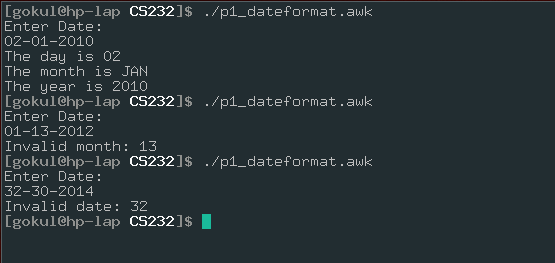
\includegraphics[width=0.9\textwidth]{img/p20.png}\newline

\subsection{Result}
The above program is run on Manjaro Linux running GNU Awk 5.0.1. 
Each query is checked and output is verified
\end{document}